\documentclass{beamer}

\usepackage[utf8]{inputenc}
\usepackage[T2A]{fontenc}
\usepackage[russian]{babel}

\usepackage{url}
\usepackage{qrcode}

\usepackage{amsmath}
\usepackage{tikz}
\usepackage{graphicx}
\usepackage{svg}
\usepackage{wrapfig}

\usetheme{Madrid}

\defbeamertemplate*{title page}{customized}[1][]
{
    \begingroup
    \centering
    \begin{beamercolorbox}[sep=8pt,center,rounded=true,shadow]{title}
        \usebeamerfont{title}
        \inserttitle
    \end{beamercolorbox}
    \vskip1em\par
    \hfill
    \hbox{
        \usebeamerfont{author}
        \begin{tabular}{ll}
            Студент: & Суркис Антон Игоревич \\
            Научный руководитель: & Попов Иван Александрович \\
        \end{tabular}
    }
    \vskip1em\par
    \begin{beamercolorbox}[sep=8pt,center,#1]{institute}
        % \usebeamerfont{institute}
        \insertinstitute
    \end{beamercolorbox}
    \begin{beamercolorbox}[sep=8pt,center,#1]{date}
        \usebeamerfont{date}\insertdate
    \end{beamercolorbox}\vskip0.5em
    {\usebeamercolor[fg]{titlegraphic}\inserttitlegraphic\par}
    \endgroup
}

\title[Ограничения Nanite]{Исследование ограничений процедурного кластерного видозависимого лоддирования в современных компьютерных играх}
\author{Антон Суркис}
\institute{Университет ИТМО}

\begin{document}
    \begin{frame}
        \titlepage
        \thispagestyle{empty}
    \end{frame}
    \clearpage
\section{ВВЕДЕНИЕ}
Наиболее распространённый метод изображения любого объекта в трёхмерных компьютерных играх --- отрисовка набора треугольников, проецируемых из виртуального трёхмерного пространства на экран.
Такой набор треугольников называется ,,мешем`` --- транслитерация устоявшегося английского термина mesh, обычно меш задаёт приближение поверхности объекта.
Целевые платформы компьютерных игр, компьютеры и игровые приставки, оснащены видеокартами --- сопроцессорами, аппаратно поддерживающими быструю отрисовку мешей.

На рисунках~\ref{fig:mesh-example-wireframe} и~\ref{fig:mesh-example-solid} приведён пример меша в виде рёбер треугольников и самих треугольников соответственно.

\begin{figure}[H]
    \centering
    \includegraphics[width=\textwidth]{pics/mesh-example-wireframe.png}
    \caption{Пример меша}
    \label{fig:mesh-example-wireframe}
\end{figure}

\begin{figure}[H]
    \centering
    \includegraphics[width=\textwidth]{pics/mesh-example-solid.png}
    \caption{Пример меша}
    \label{fig:mesh-example-solid}
\end{figure}

Для большей правдоподобности изображения компьютерные игры стремятся увеличивать разрешение мешей --- приближать поверхность объекта большим количеством треугольников малого размера.
Во многих случаях меши, применяемые в программе, составляются из исходных мешей высокого разрешения, например, отсканированных реальных объектов.

Для компьютерных игр критически важно выводить изображение в реальном времени, т.к. оно является реакцией на пользовательский ввод.
Вычислительных мощностей современных компьютеров хватает, чтобы выводить на экран в реальном времени около 20 млн. треугольников суммарно.
Как правило, один объект не будет превышать такого порога, но в области видимости могут находиться сотни объектов одновременно, и если каждый из них содержит по 10 млн. треугольников, то отрисовывать их в реальном времени будет невозможно.

Классическое решение вышеупомянутой проблемы состоит в отрисовке объектов с разными уровнями детализации.
Уровни детализации, также называемые ,,лодами`` от английской аббревиатуры LOD (level of detail) --- это набор мешей одного и того же объекта в разных разрешениях.
Уровень детализации для отрисовки объекта выбирается на основании оценки визуального искажения данного уровня детализации с учётом положения объекта относительно камеры.
Например, для объекта, расположенного вплотную к камере, будет отрисован меш в максимальном разрешении, а для объекта далеко от камеры можно использовать низкий уровень детализации.
Такое решение далее в работе будет называться монолитным лоддированием или монолитной детализацией.

У алгоритмов, использующих уровни детализации, есть значительные проблемы: создание лодов требует ручной доработки, а подбор порогов переключения между лодами выполняется вручную.
Также существуют крупные объекты, такие как статуи, скалы и здания, для которых выбор уровня детализации неоднозначен, например, если игрок рассматривает кирпичную стену здания вблизи, то ему должны быть видны мельчайшие детали вплоть до царапин на кирпичах, но для этого здание целиком нужно рисовать в максимальном разрешении, включая ту часть стены, которая находится от игрока на таком расстоянии, что отдельные кирпичи будут едва различимы --- это требует столько же ресурсов, как если бы были видны мельчайшие детали всей стены целиком.

Существуют разные технологии, решающие проблему уменьшения вычислительной сложности отрисовки геометрии.
Помимо алгоритмов на основе уровней детализации наиболее примечательны следующие:
\begin{itemize}
    \item Geometry Clipmaps~\cite{GPUGems2GeometryClipmaps}
    \item Sparse Voxel Octrees~\cite{SparseVoxelOctrees}
    \item Nanite~\cite{NaniteManual}
\end{itemize}

Geometry Clipmaps оптимизирует отрисовку ландшафта, используя карту высот --- растровое двумерное изображение, цвет каждого пикселя в котором соответствует некоторой высоте.
Ландшафты составляют значительную часть геометрии сцены, и Geometry Clipmaps существенно ускоряют их отрисовку, но для большинства объектов невозможно составить такую карту высот в некоторой параллельной проекции, которая однозначно описывала бы всю поверхность объекта, поэтому применение этой технологии ограничено.

Sparse Voxel Octrees вместо описания поверхности объекта, которым является меш, использует описание объёма, приближая его элементарными единицами объёма --- вокселями.
Воксели являются кубическими ячейками трёхмерной сетки с малым шагом, например, 100~мкм.
Иллюстрация Sparse Voxel Octree~\cite{WikipediaSparseVoxelOctreeExample} приведена на рисунке~\ref{fig:SVO-voxel-snowman-slice-01}.

\begin{figure}[H]
    \centering
    \includegraphics[width=5cm]{pics/SVO-voxel-snowman-slice-01.png}
    \caption{Срез Sparse Voxel Octree}
    \label{fig:SVO-voxel-snowman-slice-01}
\end{figure}

Основным недостатком Sparse Voxel Octrees является существенная потеря детализации по сравнению с мешами при условии сравнимого размера сжатой записи.

В 2020 году компания Epic Games представила свой подход к уменьшению сложности вычислений при отрисовке высокодетализированных объектов --- технологию Nanite в движке Unreal Engine~5.
Nanite --- технология процедурного кластерного видозависимого изменения детализации, то есть:
\begin{itemize}
    \item Nanite автоматически создаёт уровни детализации, без необходимости дорабатывать их вручную;
    \item Nanite отображает части одного объекта с разными подходящими уровнями детализации;
    \item Nanite делает швы между разными уровнями детализации незаметными;
    \item Nanite использует меш максимально возможного разрешения, для которого хватает разрешения экрана и разрешения исходного меша.
\end{itemize}

Несмотря на заявленные преимущества и то, что исходный код Nanite открыт, подобную технологию на момент написания работы в 2024 году не внедрила ни одна из ведущих компаний, таких как:
\begin{itemize}
    \item Unity
    \item Activision
    \item Ubisoft
    \item Crytek
    \item CD Projekt Red
    \item и т.д.
\end{itemize}
Epic Games остаётся единственной компанией, успешно внедрившей технологию процедурного кластерного видозависимого изменения детализации.
Следовательно, у технологии есть какие-то существенные ограничения, сравнимые с преимуществами.

Целью выпускной квалификационной работы является демонстрация технологии процедурного кластерного видозависимого лоддирования и определение её ограничений.

Для достижения этой цели поставлены следующие задачи:
\begin{enumerate}
    \item изучить механизм работы Nanite;
    \item реализовать упрощённую систему процедурного кластерного видозависимого изменения детализации
    \begin{itemize}
        % \item одна из гипотез --- Nanite очень сложен в реализации, для её проверки предлагается реализовать упрощённую версию;
        \item упрощённая версия позволит проводить объяснимые сравнения с классической реализацией;
    \end{itemize}
    \item определить проблемы, возникающие при реализации;
    \item определить принципиальные ограничения технологии;
    \item сравнить с монолитной детализацией.
\end{enumerate}

Информация о технических и принципиальных ограничениях позволит Saber Interactive принять решение о реализации полной версии технологии и интеграции в существующий движок.

    \begin{frame}{Nanite}
    Общий механизм работы Nanite\footnote{\url{https://advances.realtimerendering.com/s2021/Karis_Nanite_SIGGRAPH_Advances_2021_final.pdf}} состоит из двух этапов:
    \begin{itemize}
        \item Предподсчёт --- преобразование модели
        \item Непосредственно отрисовка
    \end{itemize}
\end{frame}

\begin{frame}{Nanite: предподсчёт}
    \begin{itemize}
        \item Меш разбивается на мешлеты
        \item Строится граф, в котором мешлеты --- вершины
        \item Граф похож на дерево
        \item Исходные мешлеты --- листья
        \item \alert{Свойство графа: родитель менее детализирован, чем ребёнок, с любого ракурса}
    \end{itemize}
\end{frame}

\begin{frame}{Nanite: пример предподсчёта, шаг 1}
    \centering \includesvg{metis-0.svg}
\end{frame}

\begin{frame}{Nanite: пример предподсчёта, шаг 2}
    \centering \includesvg{metis-1.svg}
\end{frame}

\begin{frame}{Nanite: пример предподсчёта, шаг 3}
    \centering \includesvg{metis-2.svg}
\end{frame}

\begin{frame}{Nanite: пример предподсчёта, шаг 4}
    \centering \includesvg{metis-3.svg}
\end{frame}

\begin{frame}{Nanite: отрисовка}
    \begin{itemize}
        \item \alert{Решения об отрисовке мешлета независимы для всех мешлетов}
        \item Массовый параллелизм
        \item Корректность благодаря свойству графа
        \item Треугольники в 1 пиксель обрабатываются отдельно
    \end{itemize}
\end{frame}

    \begin{frame}{Реализация упрощённой системы}
    \begin{itemize}
        \item Нужна для лучшего понимания, как работает Nanite
        \item Преобразование меша в граф --- долгий предподсчёт
        \item Разбиение меша с помощью библиотеки METIS
        \item Невозможно задать жёсткое ограничение на размер мешлета, поэтому количество мешлетов берётся с запасом
        \item Реализован алгоритм уменьшения детализации, т.к. библиотеки работают с целым мешем
        \item Отрисовка --- Mesh Shader в DirectX 12
        \item Обход всего графа для упрощения
    \end{itemize}
\end{frame}

\begin{frame}{Реализация: скриншоты}
    \begin{center}
        Разные настройки допустимого искажения для наглядности

        \medskip

        \includegraphics[width=.2\textwidth]{pics/demo-cut-0.png}
        \includegraphics[width=.2\textwidth]{pics/demo-cut-1.png}
        \includegraphics[width=.2\textwidth]{pics/demo-cut-2.png}
        \includegraphics[width=.2\textwidth]{pics/demo-cut-3.png}

        \parbox[l]{.4\textwidth}{
            Вид вблизи
        }
        \parbox[r]{.4\textwidth}{
            \hfill
            Вид вдали
        }
    \end{center}
\end{frame}

    \begin{frame}{Проблемы при реализации}
    \begin{itemize}
        \item Разбиение на мешлеты --- NP-трудная задача
        \item Из-за этого алгоритмы --- приближения
        \item Ограничение размера мешлета
    \end{itemize}
\end{frame}

\begin{frame}{Проблемы при реализации: мешлеты}
    \includegraphics[width=\textwidth]{sphere0.png}
\end{frame}

\begin{frame}{Проблемы при реализации: последствия}
    \includegraphics[width=\textwidth]{sphere1.png}
\end{frame}

    \begin{frame}{Принципиальные ограничения}
    \begin{itemize}
        \item Оценка искажения не зависит от направления
        \item Невозможна анимация
        \item Некоторые меши так не сжимаются
    \end{itemize}
\end{frame}

\begin{frame}{Принципиальное ограничение: объём}
    \includegraphics[width=\textwidth]{plane0.png}
\end{frame}

\begin{frame}{Принципиальное ограничение: объём}
    \includegraphics[width=\textwidth]{plane1.png}
\end{frame}

    \begin{frame}{Сравнение с монолитной детализацией}
    \begin{itemize}
        \item Сравнимое качество картинки (определяется на глаз)
        \item Метрики --- FPS и количество отправляемых на растеризацию треугольников
    \end{itemize}

    \begin{center}
        \begin{tabular}{lrrr}
            \hline \hline
            Тип отрисовки & FPS & Треугольников \\ \hline
            Наивысшее разрешение & 5.4 & 640 000 000 \\
            Монолитные лоды & \textbf{114.2} & 28 900 000 \\
            Кластерные лоды & 35.0 & 58 677 326 \\
            \hline
            UE5, монолитные лоды & 61.8 & Не измерялось \\
            UE5, Nanite & \textbf{88.6} & Не измерялось \\
            \hline \hline
        \end{tabular}
    \end{center}

    \alert{Производительность кластерных лодов пока недостаточна}
\end{frame}

\begin{frame}{Упрощённая реализация и UE5}
    \begin{minipage}{.45\textwidth}
        \centering
        \includegraphics[width=\textwidth]{../Text/pics/comparison-cluster.png}

        Упрощённая реализация
    \end{minipage}
    \begin{minipage}{.45\textwidth}
        \centering
        \includegraphics[width=\textwidth]{pics/ue5-nanite.png}

        Nanite, Unreal Engine 5
    \end{minipage}

    \bigskip

    Нельзя сравнивать напрямую, но можно видеть, что Nanite лучше себя показывает по сравнению с монолитными лодами в UE5, чем упрощённая реализация --- по сравнению с простыми монолитными лодами
\end{frame}

% \begin{frame}{Сравнение с монолитной детализацией}
%     \begin{center}
%         \begin{minipage}{.45\textwidth}
%             \begin{center}
%                 \includegraphics[width=\textwidth]{../Text/pics/comparison-mono.png}

%                 Монолитные лоды
%             \end{center}
%         \end{minipage}
%         \begin{minipage}{.45\textwidth}
%             \begin{center}
%                 \includegraphics[width=\textwidth]{../Text/pics/comparison-cluster.png}

%                 Кластерные лоды
%             \end{center}
%         \end{minipage}
%         \begin{minipage}{.45\textwidth}
%             \begin{center}
%                 \includegraphics[width=\textwidth]{../Text/pics/comparison-0.png}

%                 Наивысшая детализация
%             \end{center}
%         \end{minipage}
%     \end{center}
% \end{frame}

\begin{frame}{Плотность треугольников}
    \begin{center}
        \begin{minipage}{.45\textwidth}
            \begin{center}
                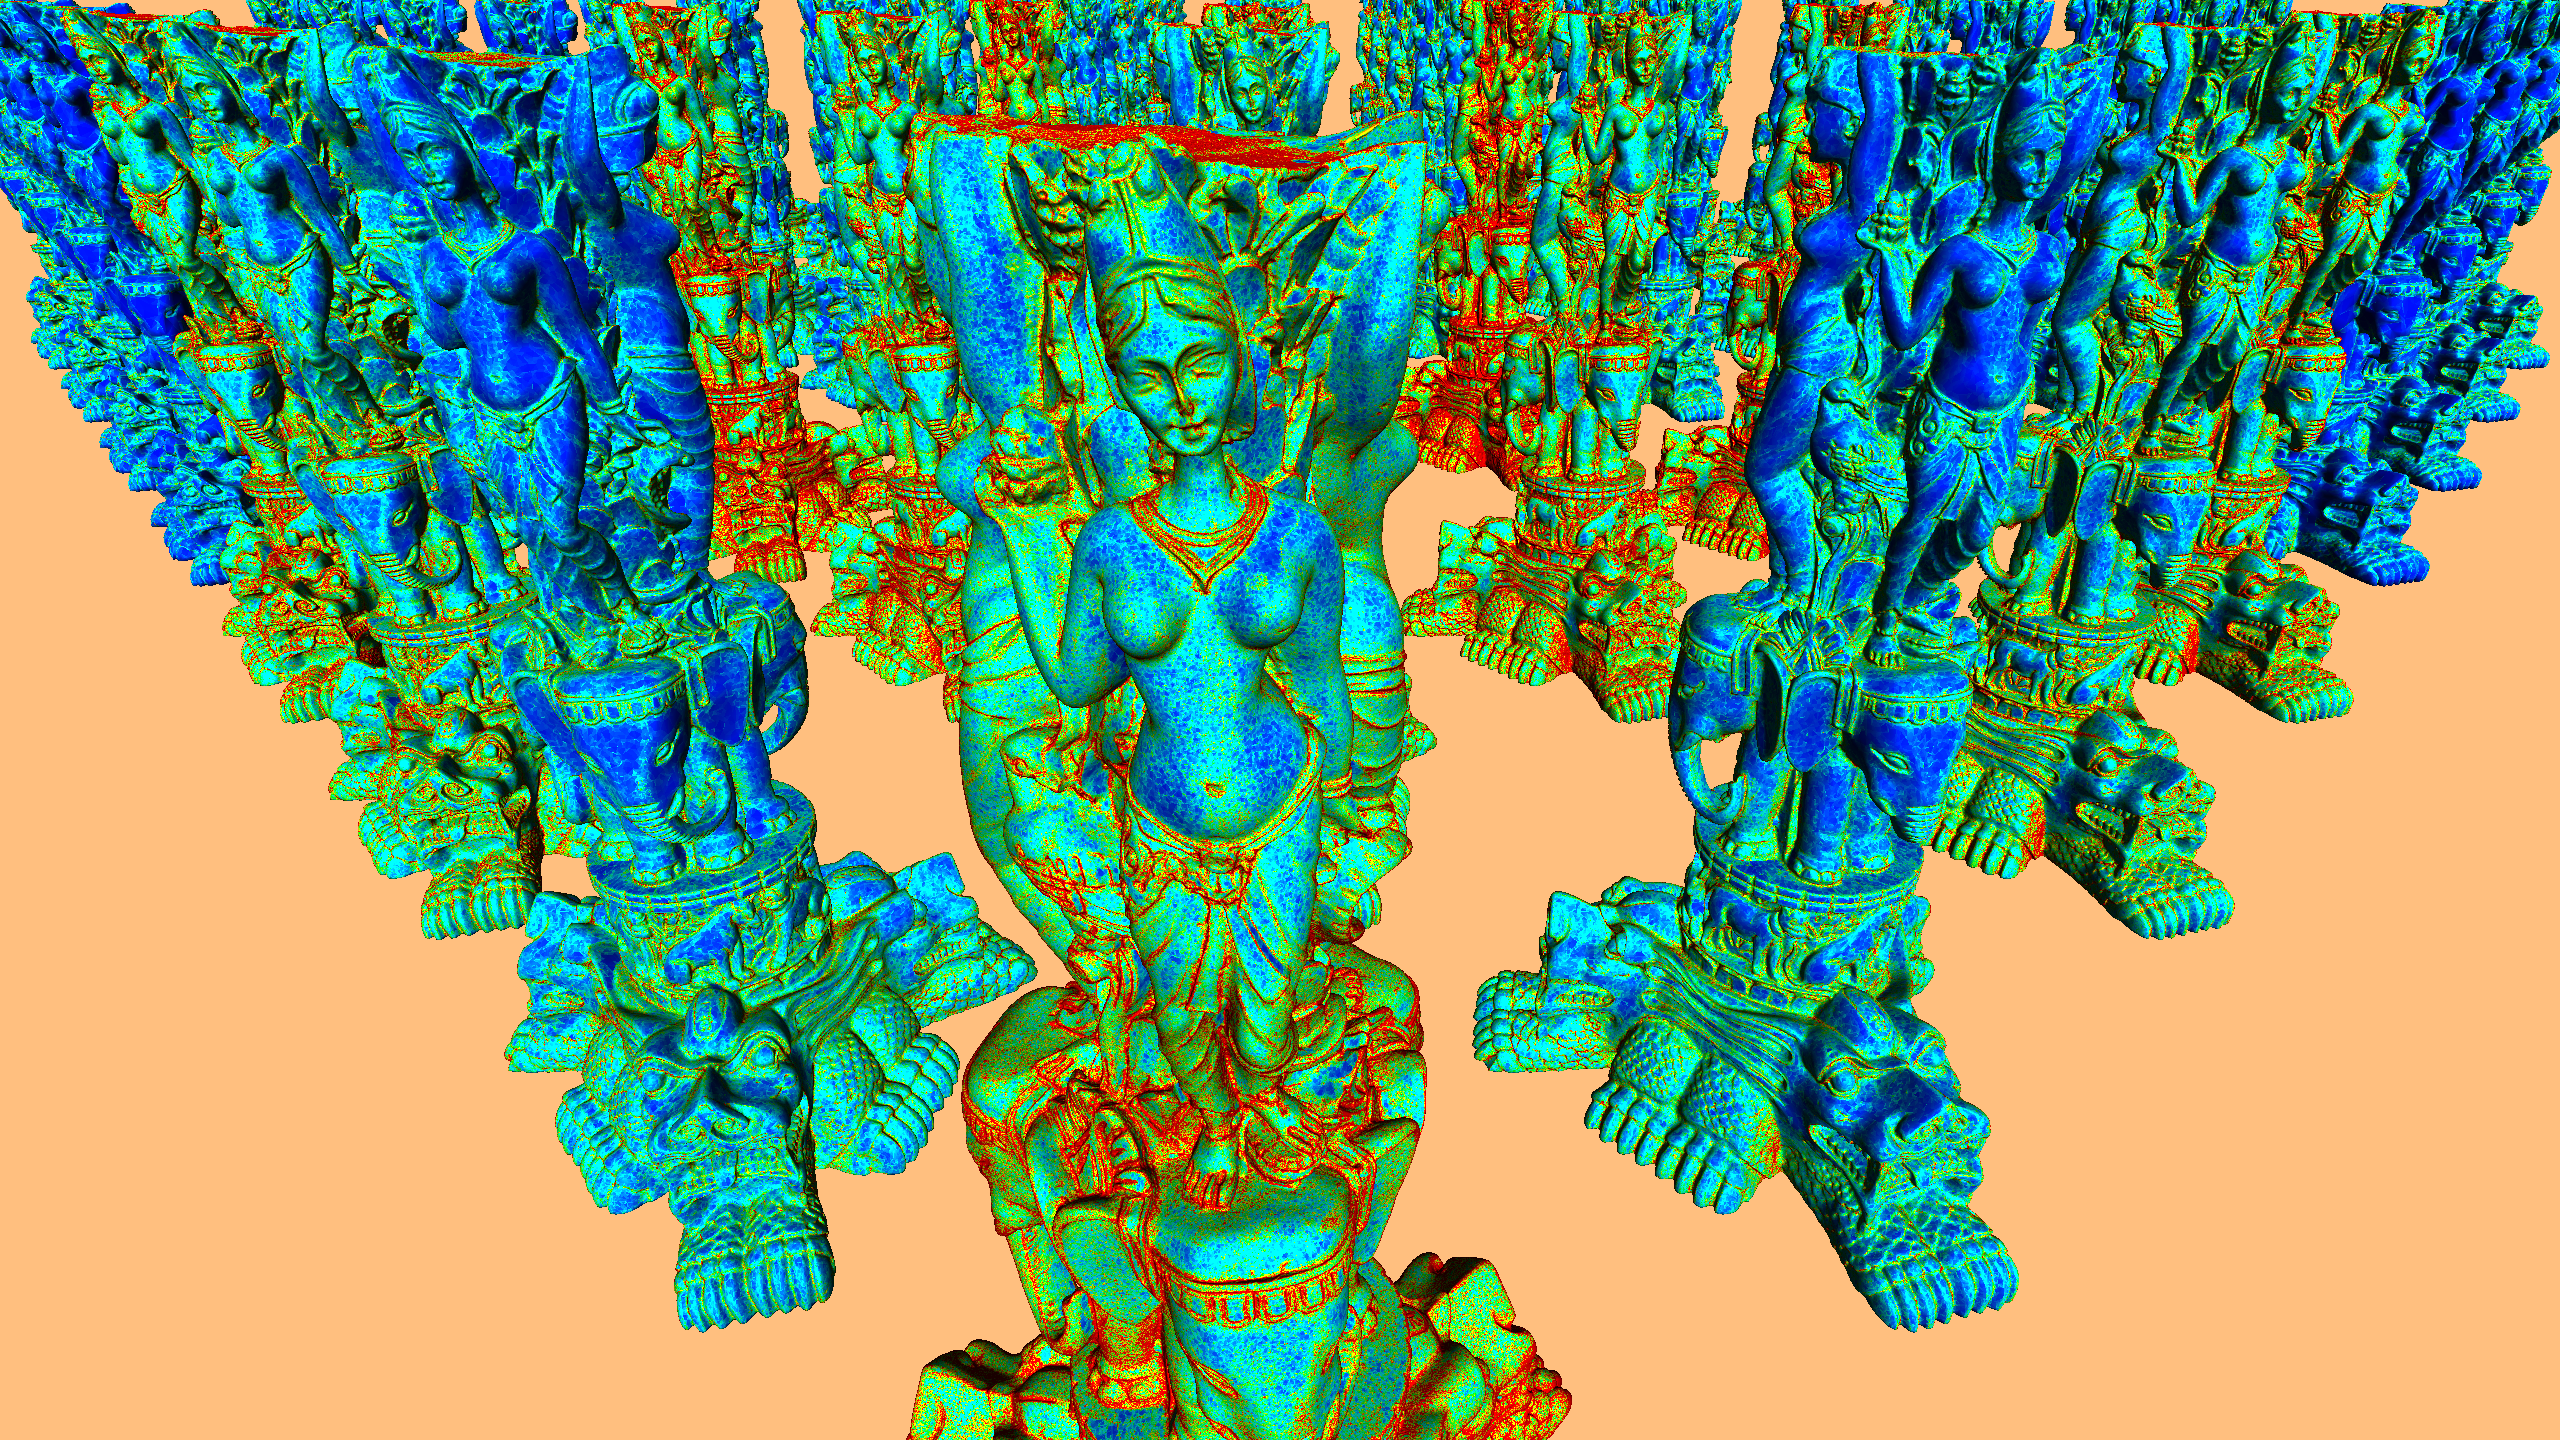
\includegraphics[width=\textwidth]{../Text/pics/heatmap-mono.png}

                Монолитные лоды
            \end{center}
        \end{minipage}
        \begin{minipage}{.45\textwidth}
            \begin{center}
                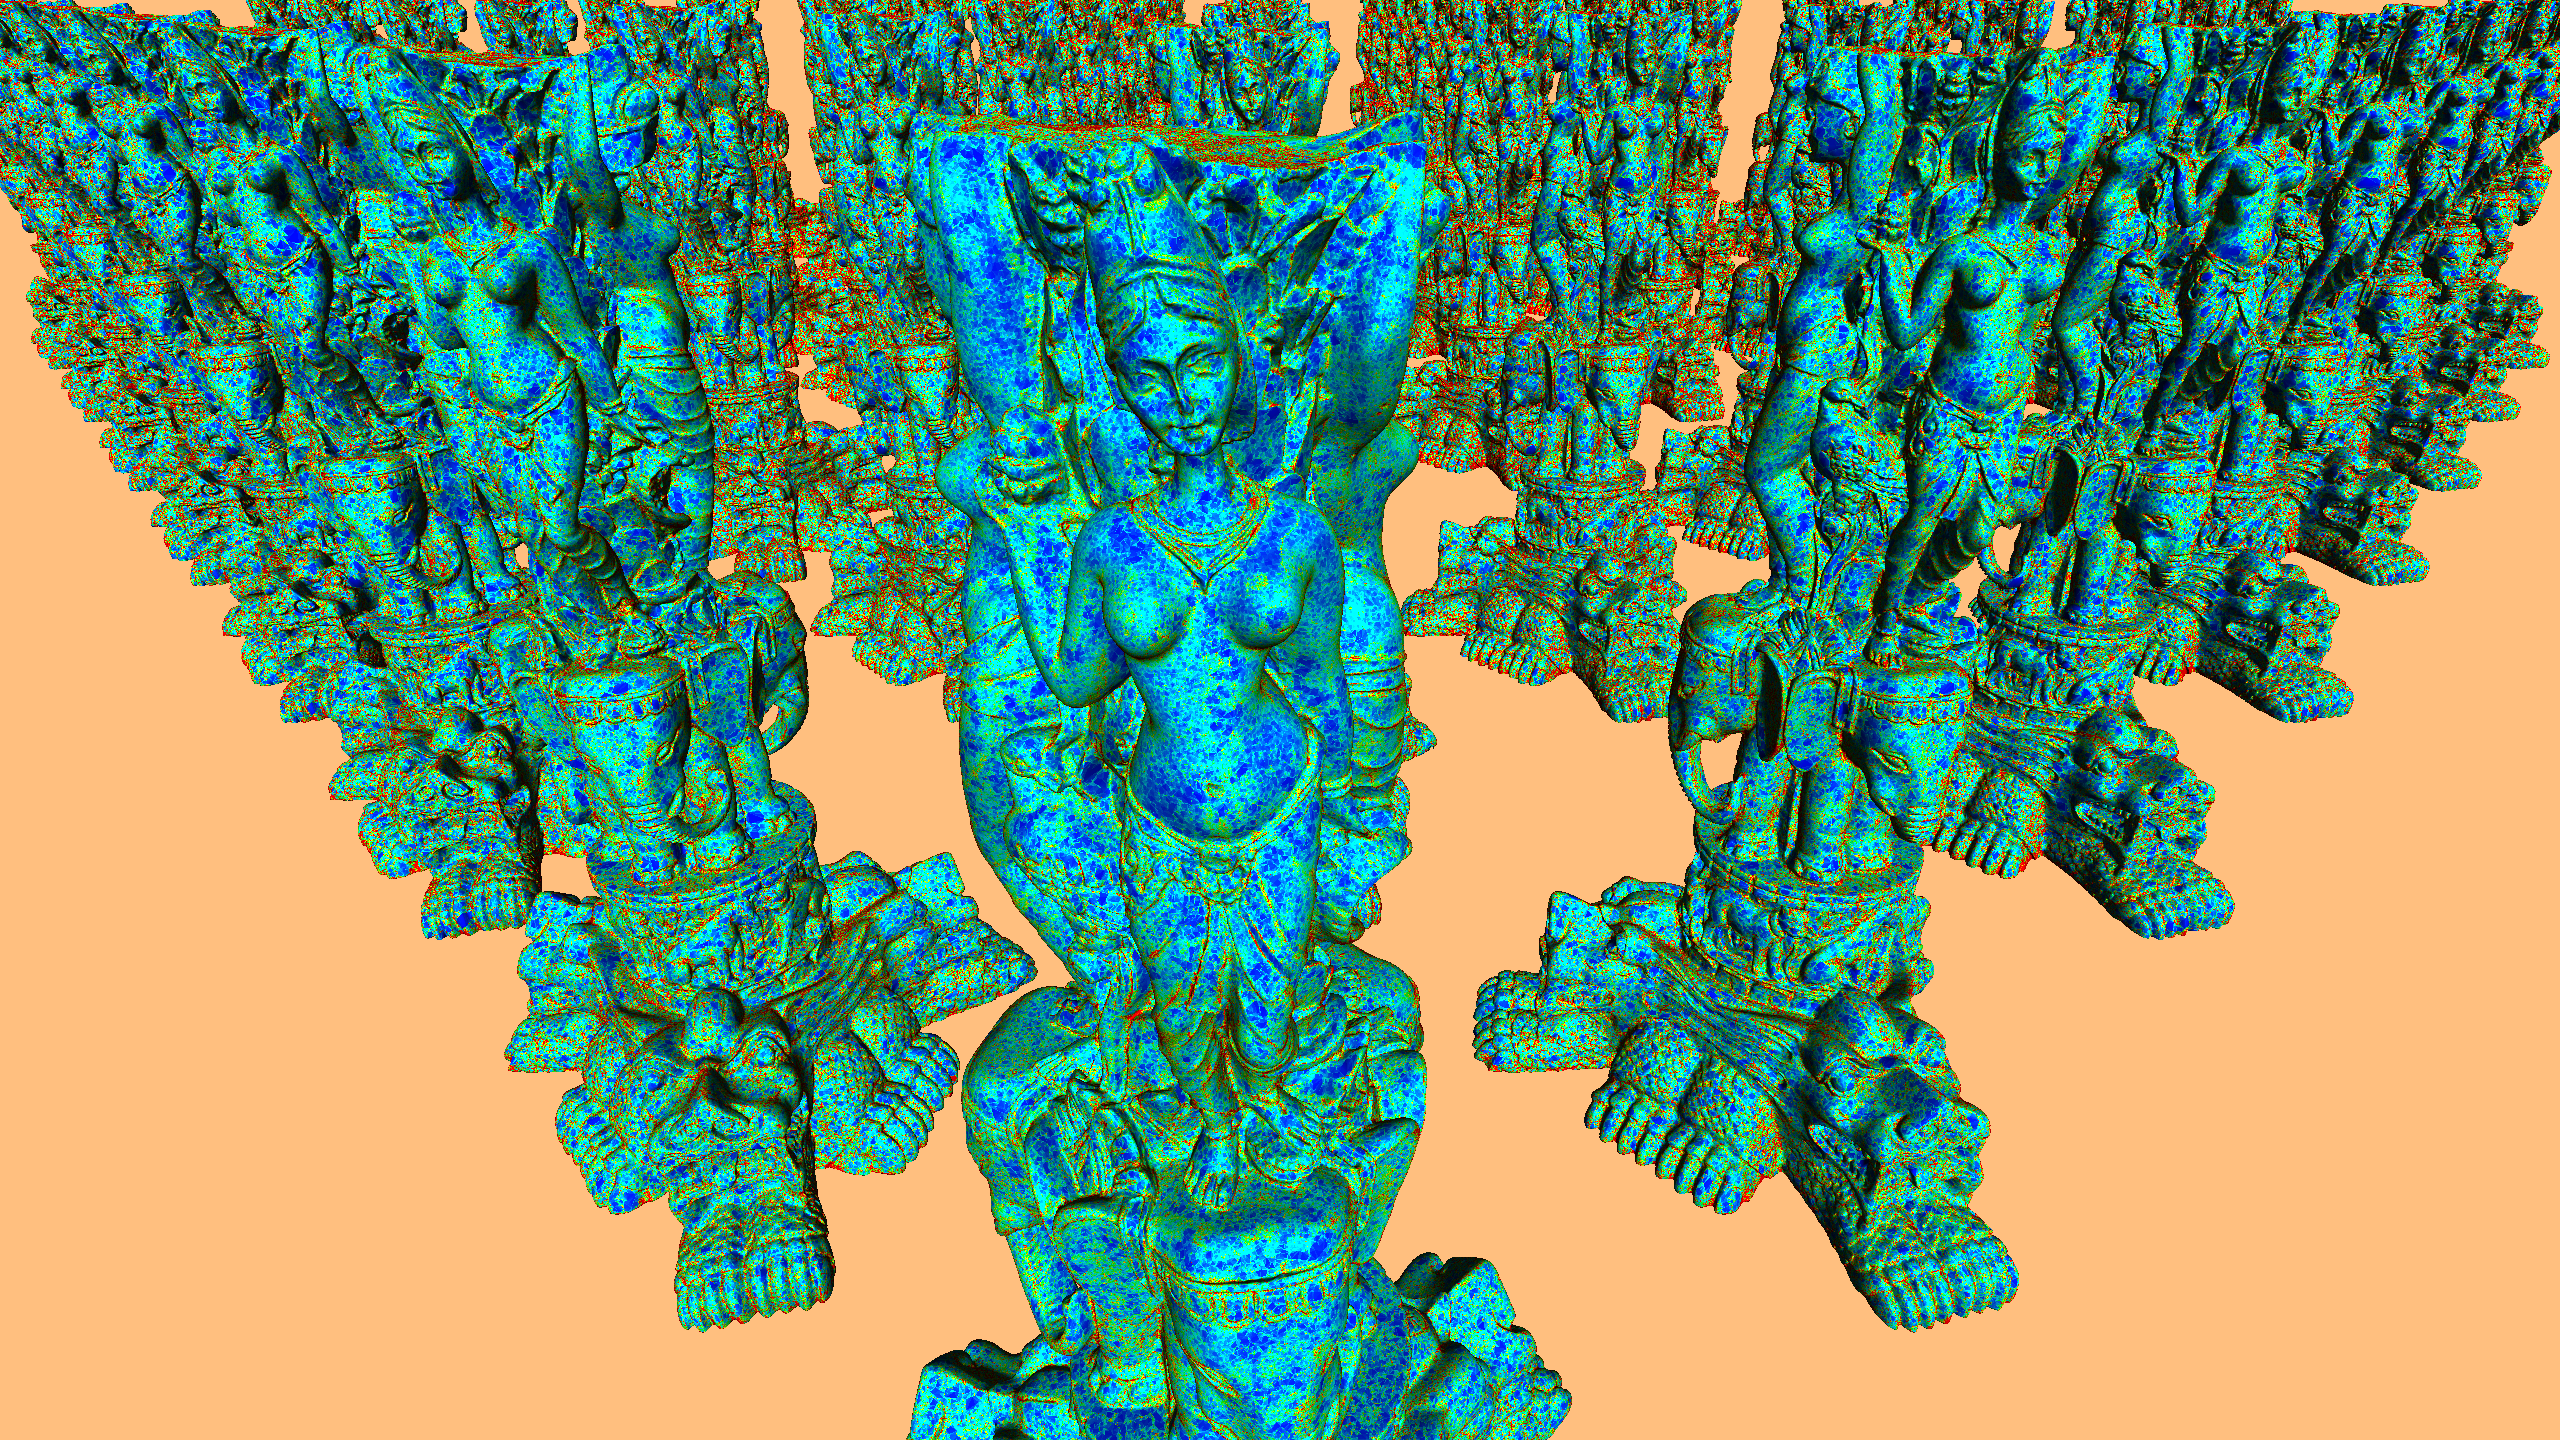
\includegraphics[width=\textwidth]{../Text/pics/heatmap-cluster.png}

                Кластерные лоды
            \end{center}
        \end{minipage}
        \begin{minipage}{.45\textwidth}
            \begin{center}
                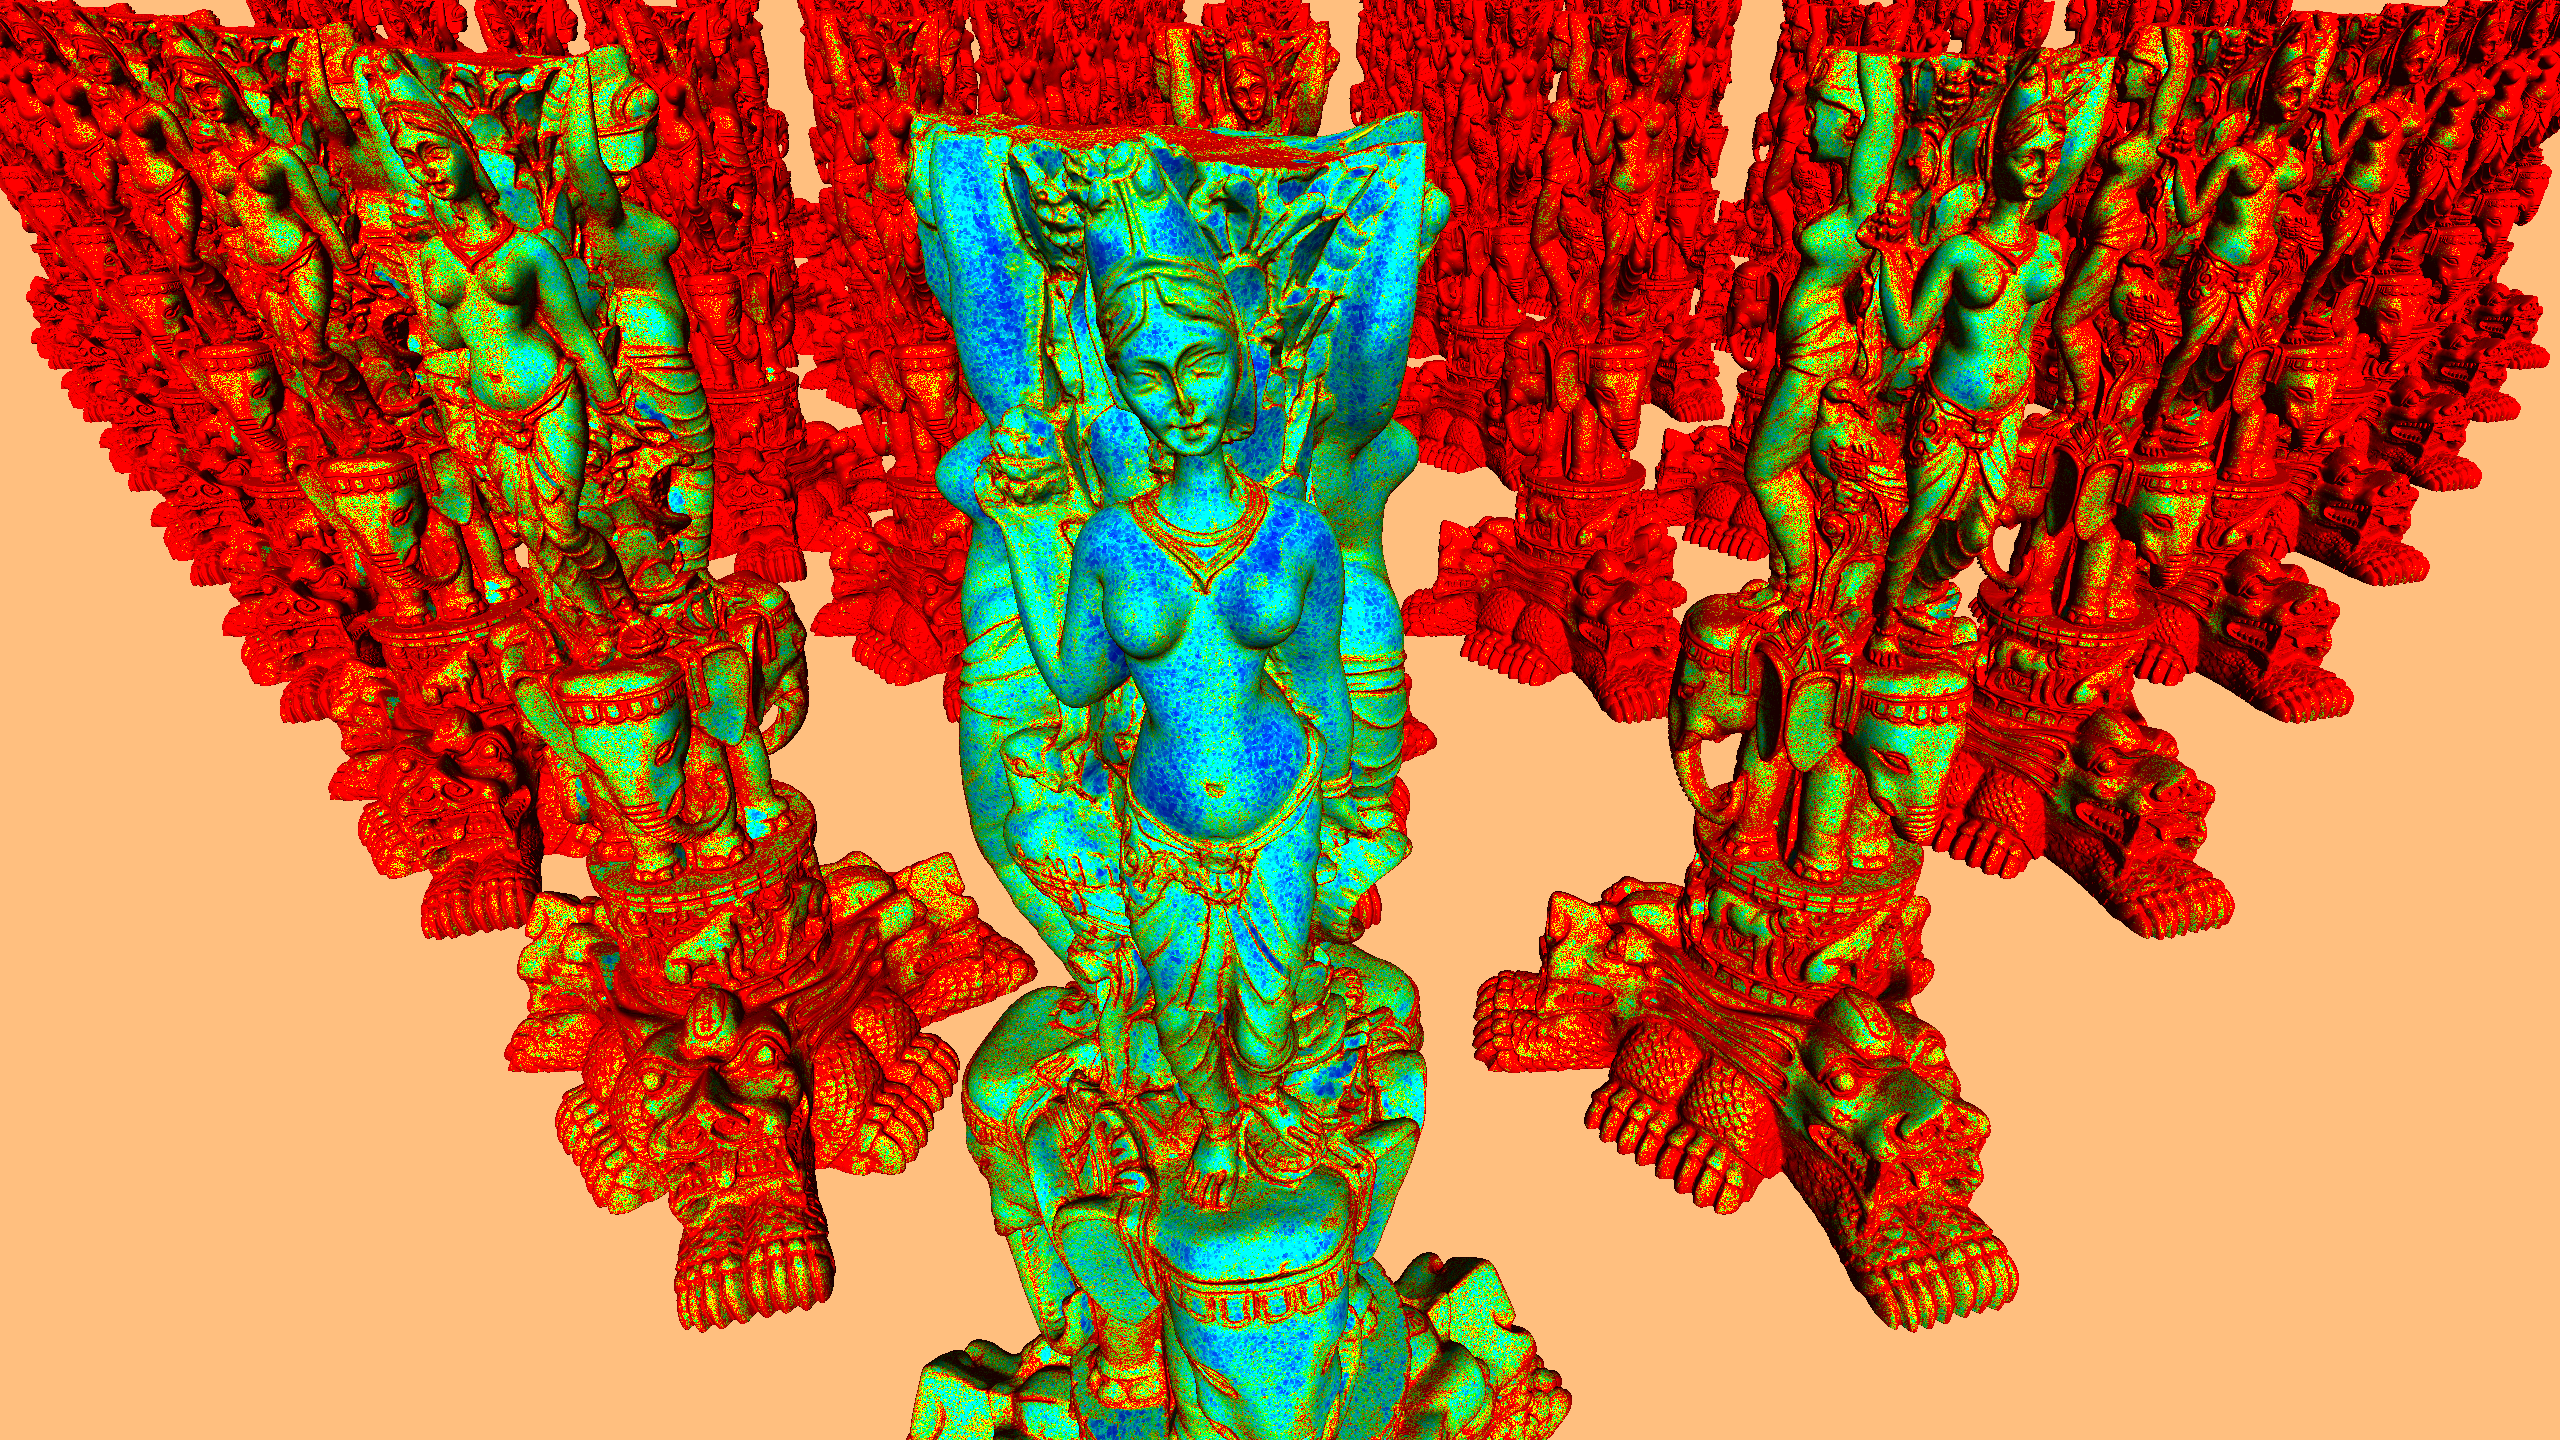
\includegraphics[width=\textwidth]{../Text/pics/heatmap-0.png}

                Наивысшая детализация
            \end{center}
        \end{minipage}
    \end{center}
\end{frame}

    \clearpage
\section{ЗАКЛЮЧЕНИЕ}
Целью выпускной квалификационной работы является демонстрация технологии процедурного кластерного видозависимого лоддирования и определение её ограничений.

Для достижения этой цели были поставлены следующие задачи:
\begin{enumerate}
    \item изучить механизм работы Nanite;
    \item реализовать упрощённую систему процедурного кластерного видозависимого изменения детализации;
    \item определить проблемы, возникающие при реализации;
    \item определить принципиальные ограничения технологии;
    \item сравнить с ,,монолитной`` детализацией.
\end{enumerate}

Для достижения цели и задач был изучен механизм работы Nanite --- первой известной успешно внедрённой в коммерческий движок реализации такой технологии.
Механизм работы Nanite основывается на преобразовании исходного меша в граф мешлетов, в котором поддерживается следующее свойство: независимо от ракурса оценка искажения мешлета-ребёнка не превышает оценку искажения мешлета-родителя.
Это свойство используется для массового параллелизма в отрисовке мешлетов разной детализации без видимых искажений.

Для лучшего понимания механизма работы Nanite реализована упрощённая версия системы и продемонстрирована корректность работы реализованной упрощённой версии, и, как следствие, технологии в целом.
В ходе реализации выявлены принципиальные ограничения такой технологии и существенные технические проблемы, которые необходимо решать при реализации полной версии.

Определены следующие технические проблемы, которые необходимо подробнее рассмотреть при реализации полной версии технологии:
\begin{itemize}
    \item задача разбиения графа;
    \item ограничение размера мешлетов;
    \item оптимизация структуры мешлетов;
    \item организация параллельного спуска по графу;
    \item организация параллельной децимации.
\end{itemize}

Определены следующие существенные принципиальные ограничения технологии, на основании которых можно определить, к каким частям проекта технология применима и потенциальные выгоды от разработки и интеграции полной версии:
\begin{itemize}
    \item оценка искажения не зависит от направления взгляда;
    \item невозможность анимации меша;
    \item неприменимость к некоторым типам мешей;
    \item необходимость использовать меши сверхвысокого разрешения.
\end{itemize}

Проведено сравнение с тривиальным алгоритмом монолитного лоддирования, это сравнение показало, что полученная реализация технологии процедурного кластерного видозависимого лоддирования пока сущетсвенно проигрывает в производительности тривиальному алгоритму монолитного лоддирования.
Для исправления этого в дальнейших работах предлагается исследовать те оптимизации, предложенные в главе 3, которые не были реализованы в данной работе.

Таким образом, поставленные задачи выполнены и поставленная цель выпускной квалификационной работы достигнута.

    \newcounter{finalframe}
    \setcounter{finalframe}{\value{framenumber}}
    \begin{frame}{Доп.: Geometry Clipmaps}
    \begin{minipage}{.5\textwidth}
        \begin{itemize}
            \item Для ландшафта можно построить растровую карту высот
            \item Уменьшение детализации растровых изображений --- хорошо изученная задача
            \item По карте высот можно без разрывов рисовать геометрию разной детализации
        \end{itemize}
    \end{minipage}
    \begin{minipage}{.45\textwidth}
        \includegraphics[width=\textwidth]{02_clipmaps_01.jpg}

        \includegraphics[width=\textwidth]{02_clipmaps_02.jpg}
    \end{minipage}
\end{frame}

\begin{frame}{Доп.: Sparse Voxel Octree}
    \centering
    \begin{minipage}{.75\textwidth}
        \begin{itemize}
            \item Меши приближают поверхность объекта
            \item Можно приближать не поверхность объекта, а его объём
            \item Воксель --- элементарная единица объёма
            \item Приближение объёма вокселями --- фактически, трёхмерное растровое изображение
            \item Одинаковые воксели группируются в кубы для экономии памяти и ускорения вычислений
        \end{itemize}
    \end{minipage}
    \begin{minipage}{.2\textwidth}
        \includegraphics[width=\textwidth]{../Text/pics/SVO-voxel-snowman-slice-01.png}
    \end{minipage}
\end{frame}

\begin{frame}{Доп.: Плотность треугольников}
    \begin{center}
        \begin{minipage}{.45\textwidth}
            \begin{center}
                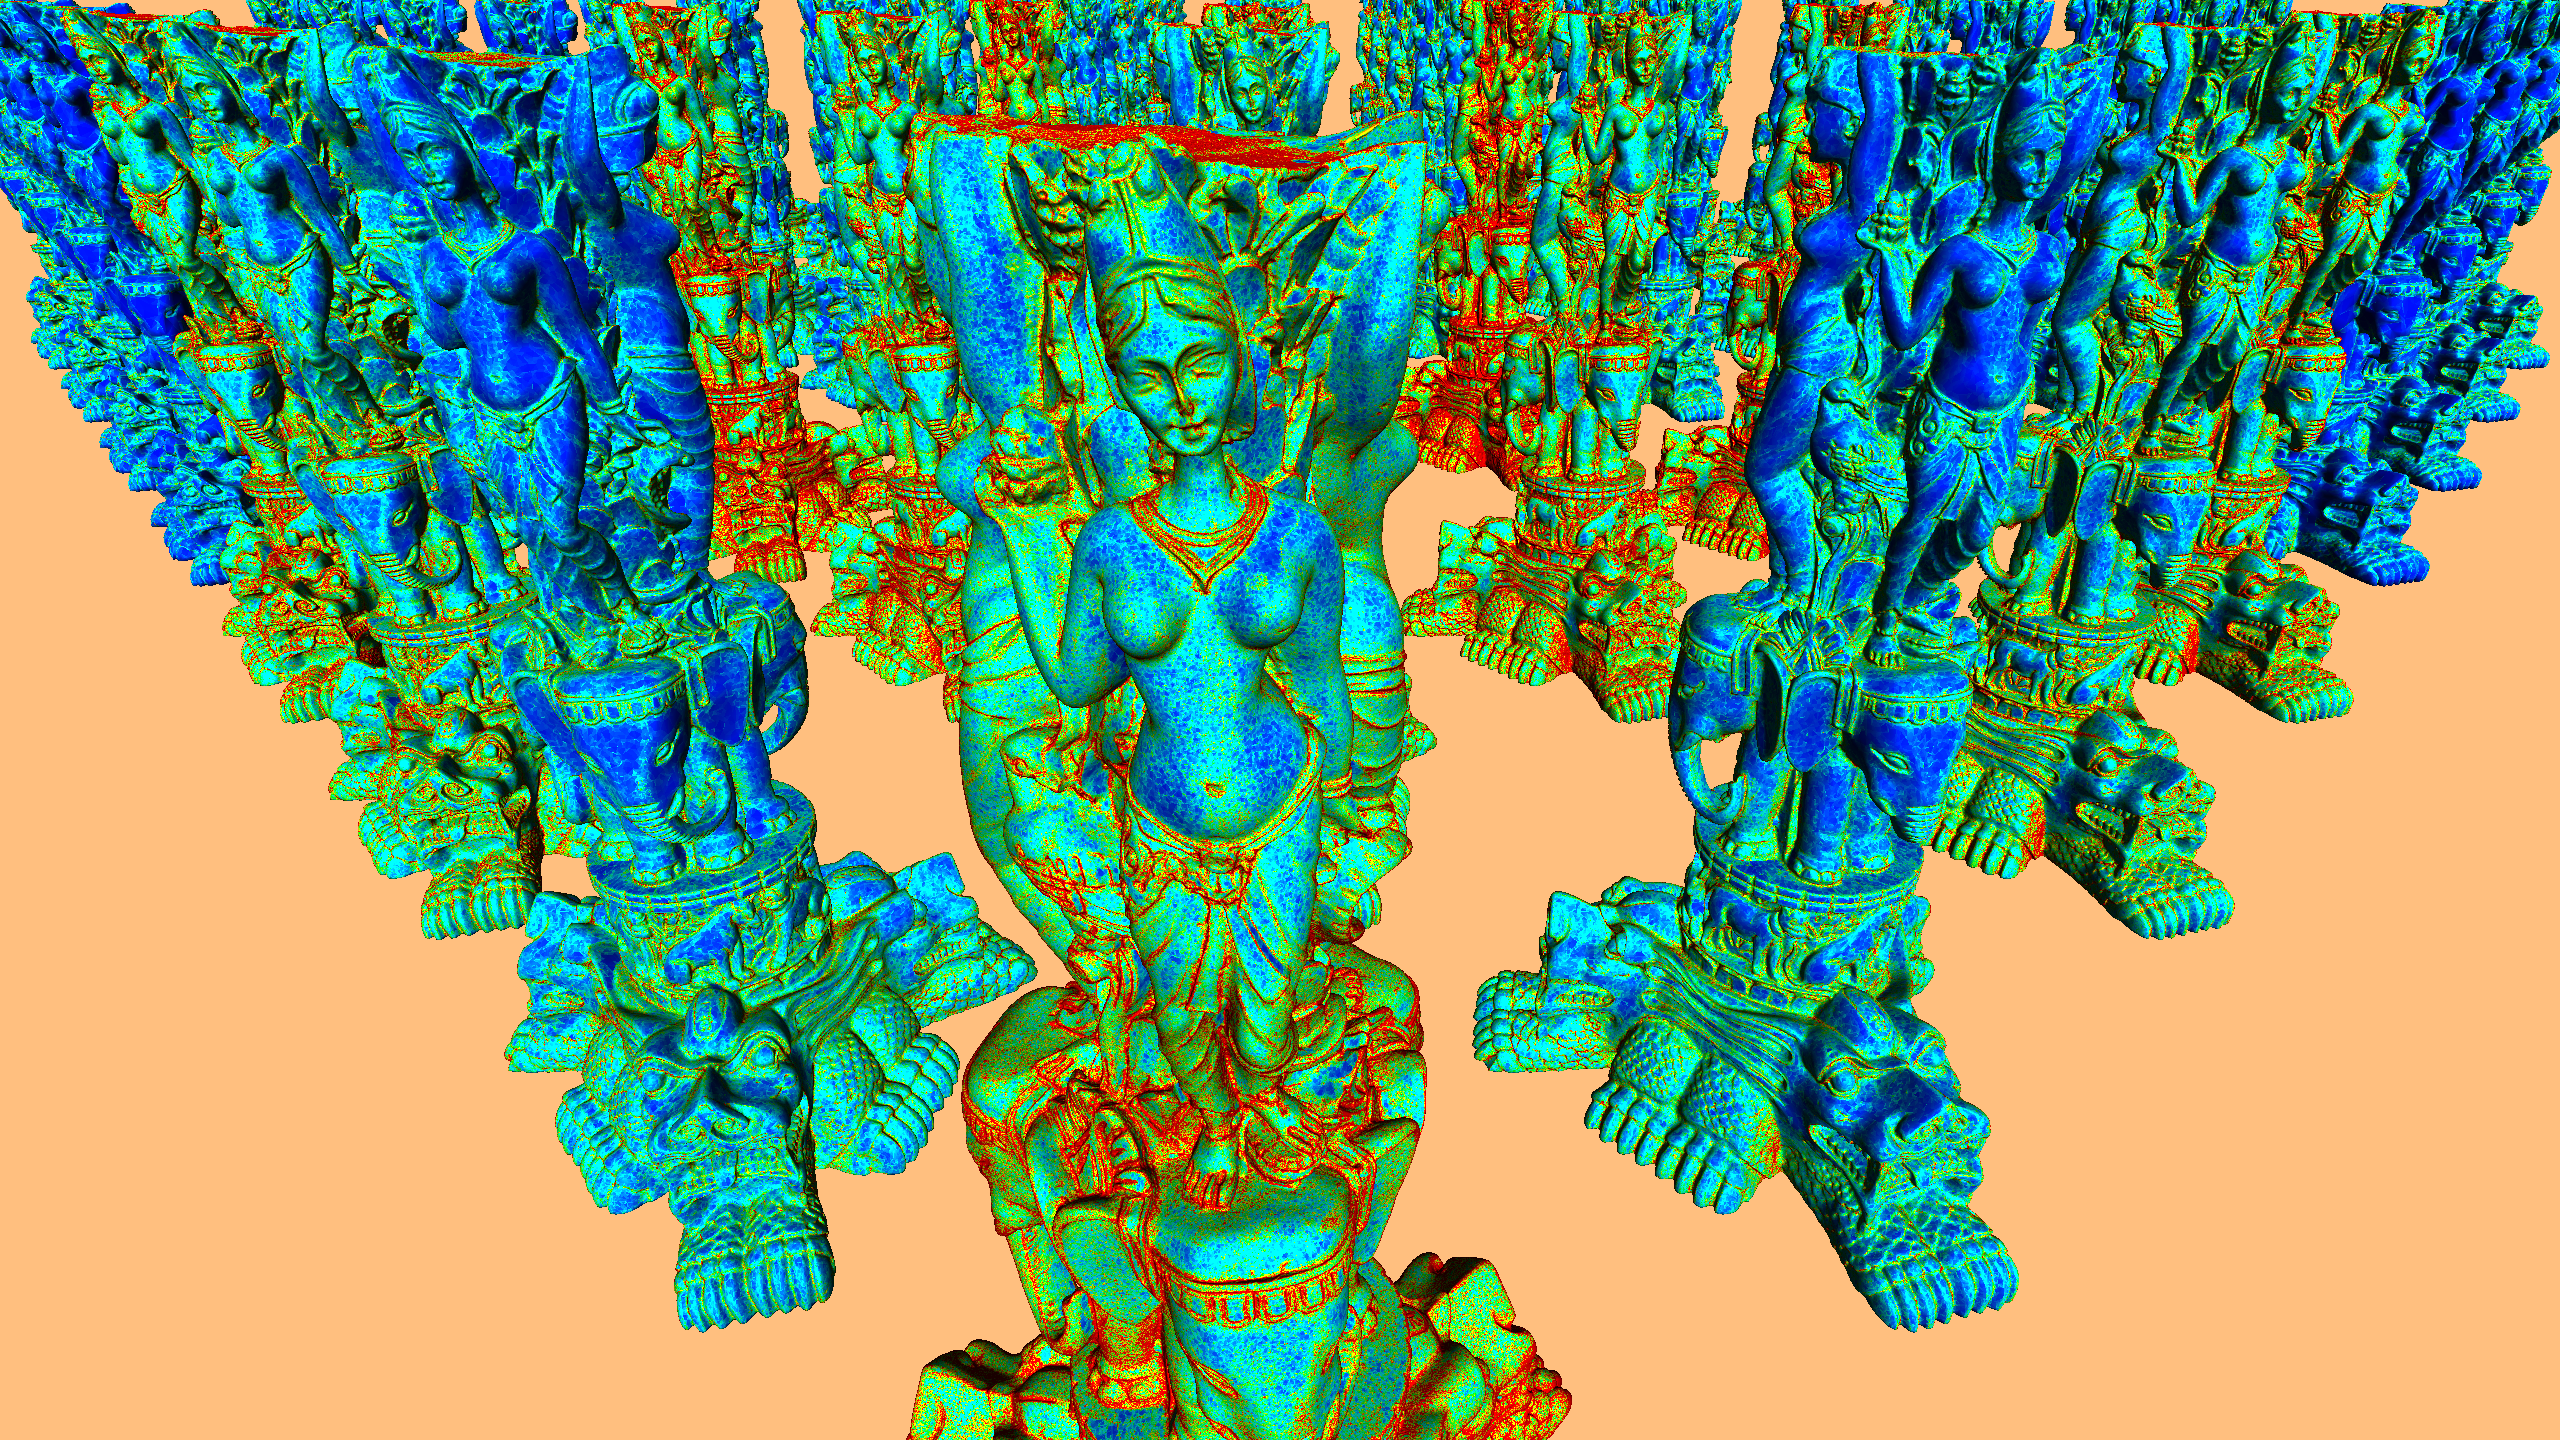
\includegraphics[width=\textwidth]{../Text/pics/heatmap-mono.png}

                Монолитные лоды
            \end{center}
        \end{minipage}
        \begin{minipage}{.45\textwidth}
            \begin{center}
                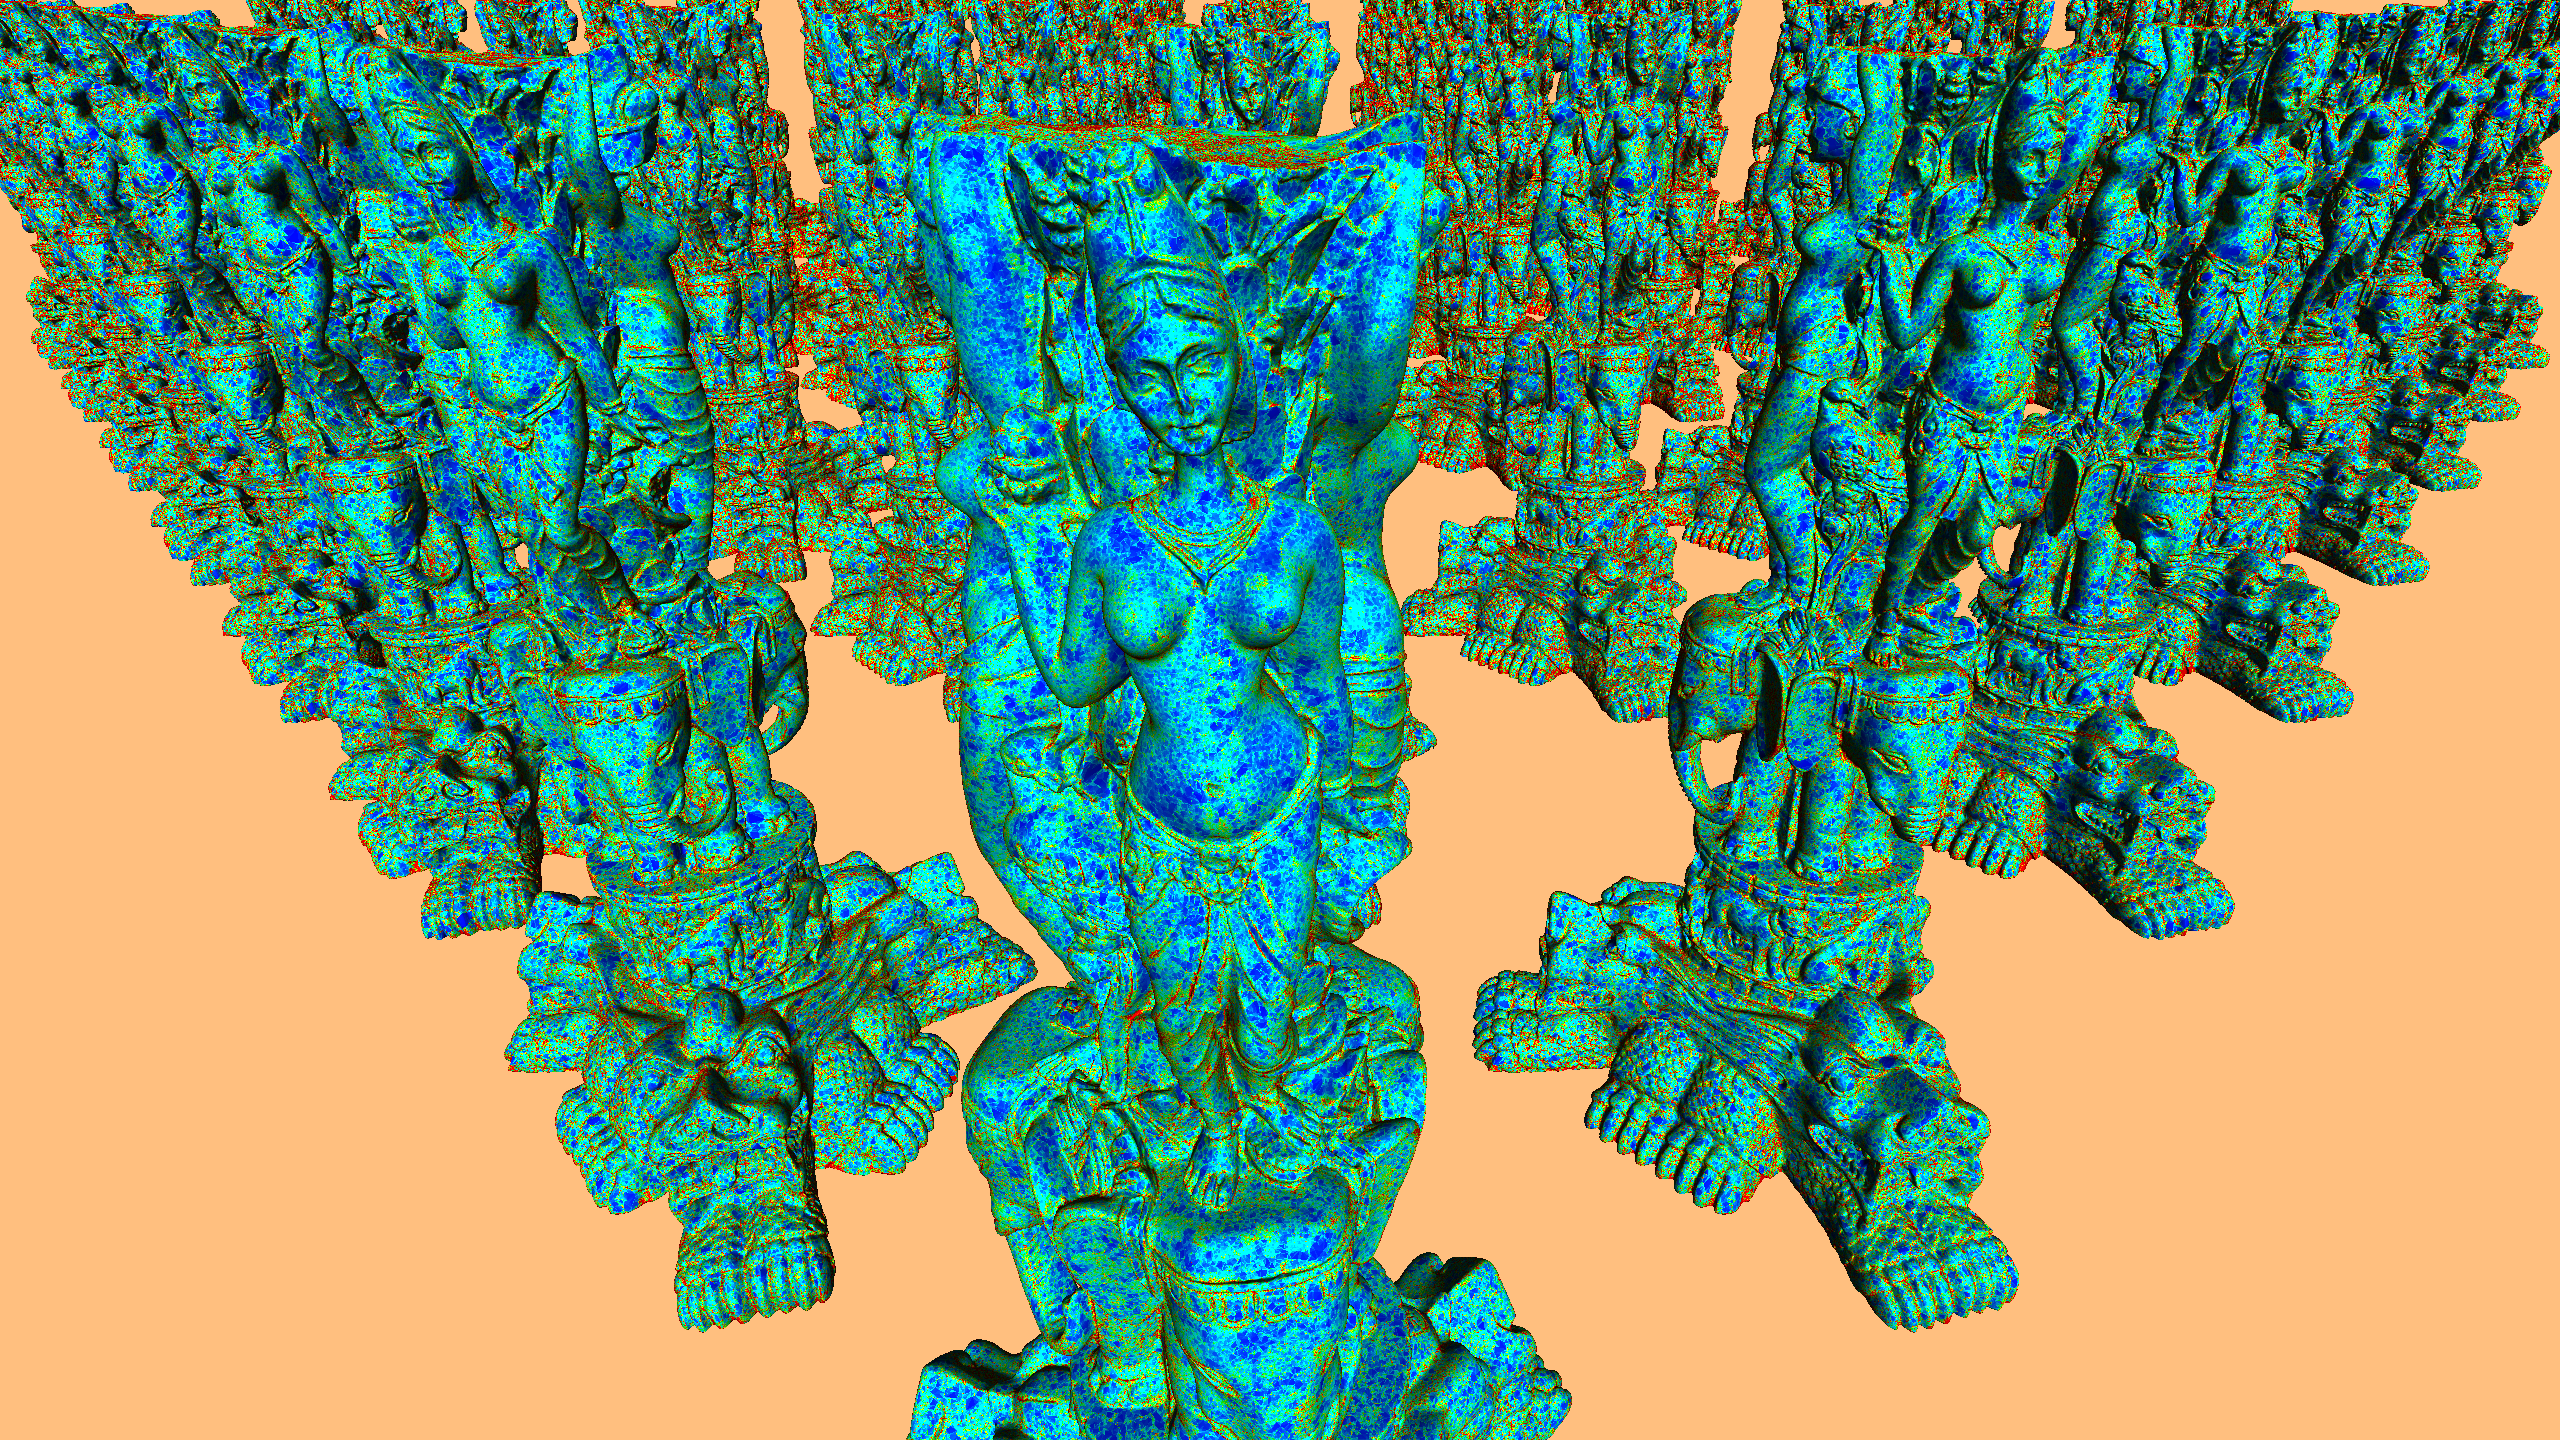
\includegraphics[width=\textwidth]{../Text/pics/heatmap-cluster.png}

                Кластерные лоды
            \end{center}
        \end{minipage}
        \begin{minipage}{.45\textwidth}
            \begin{center}
                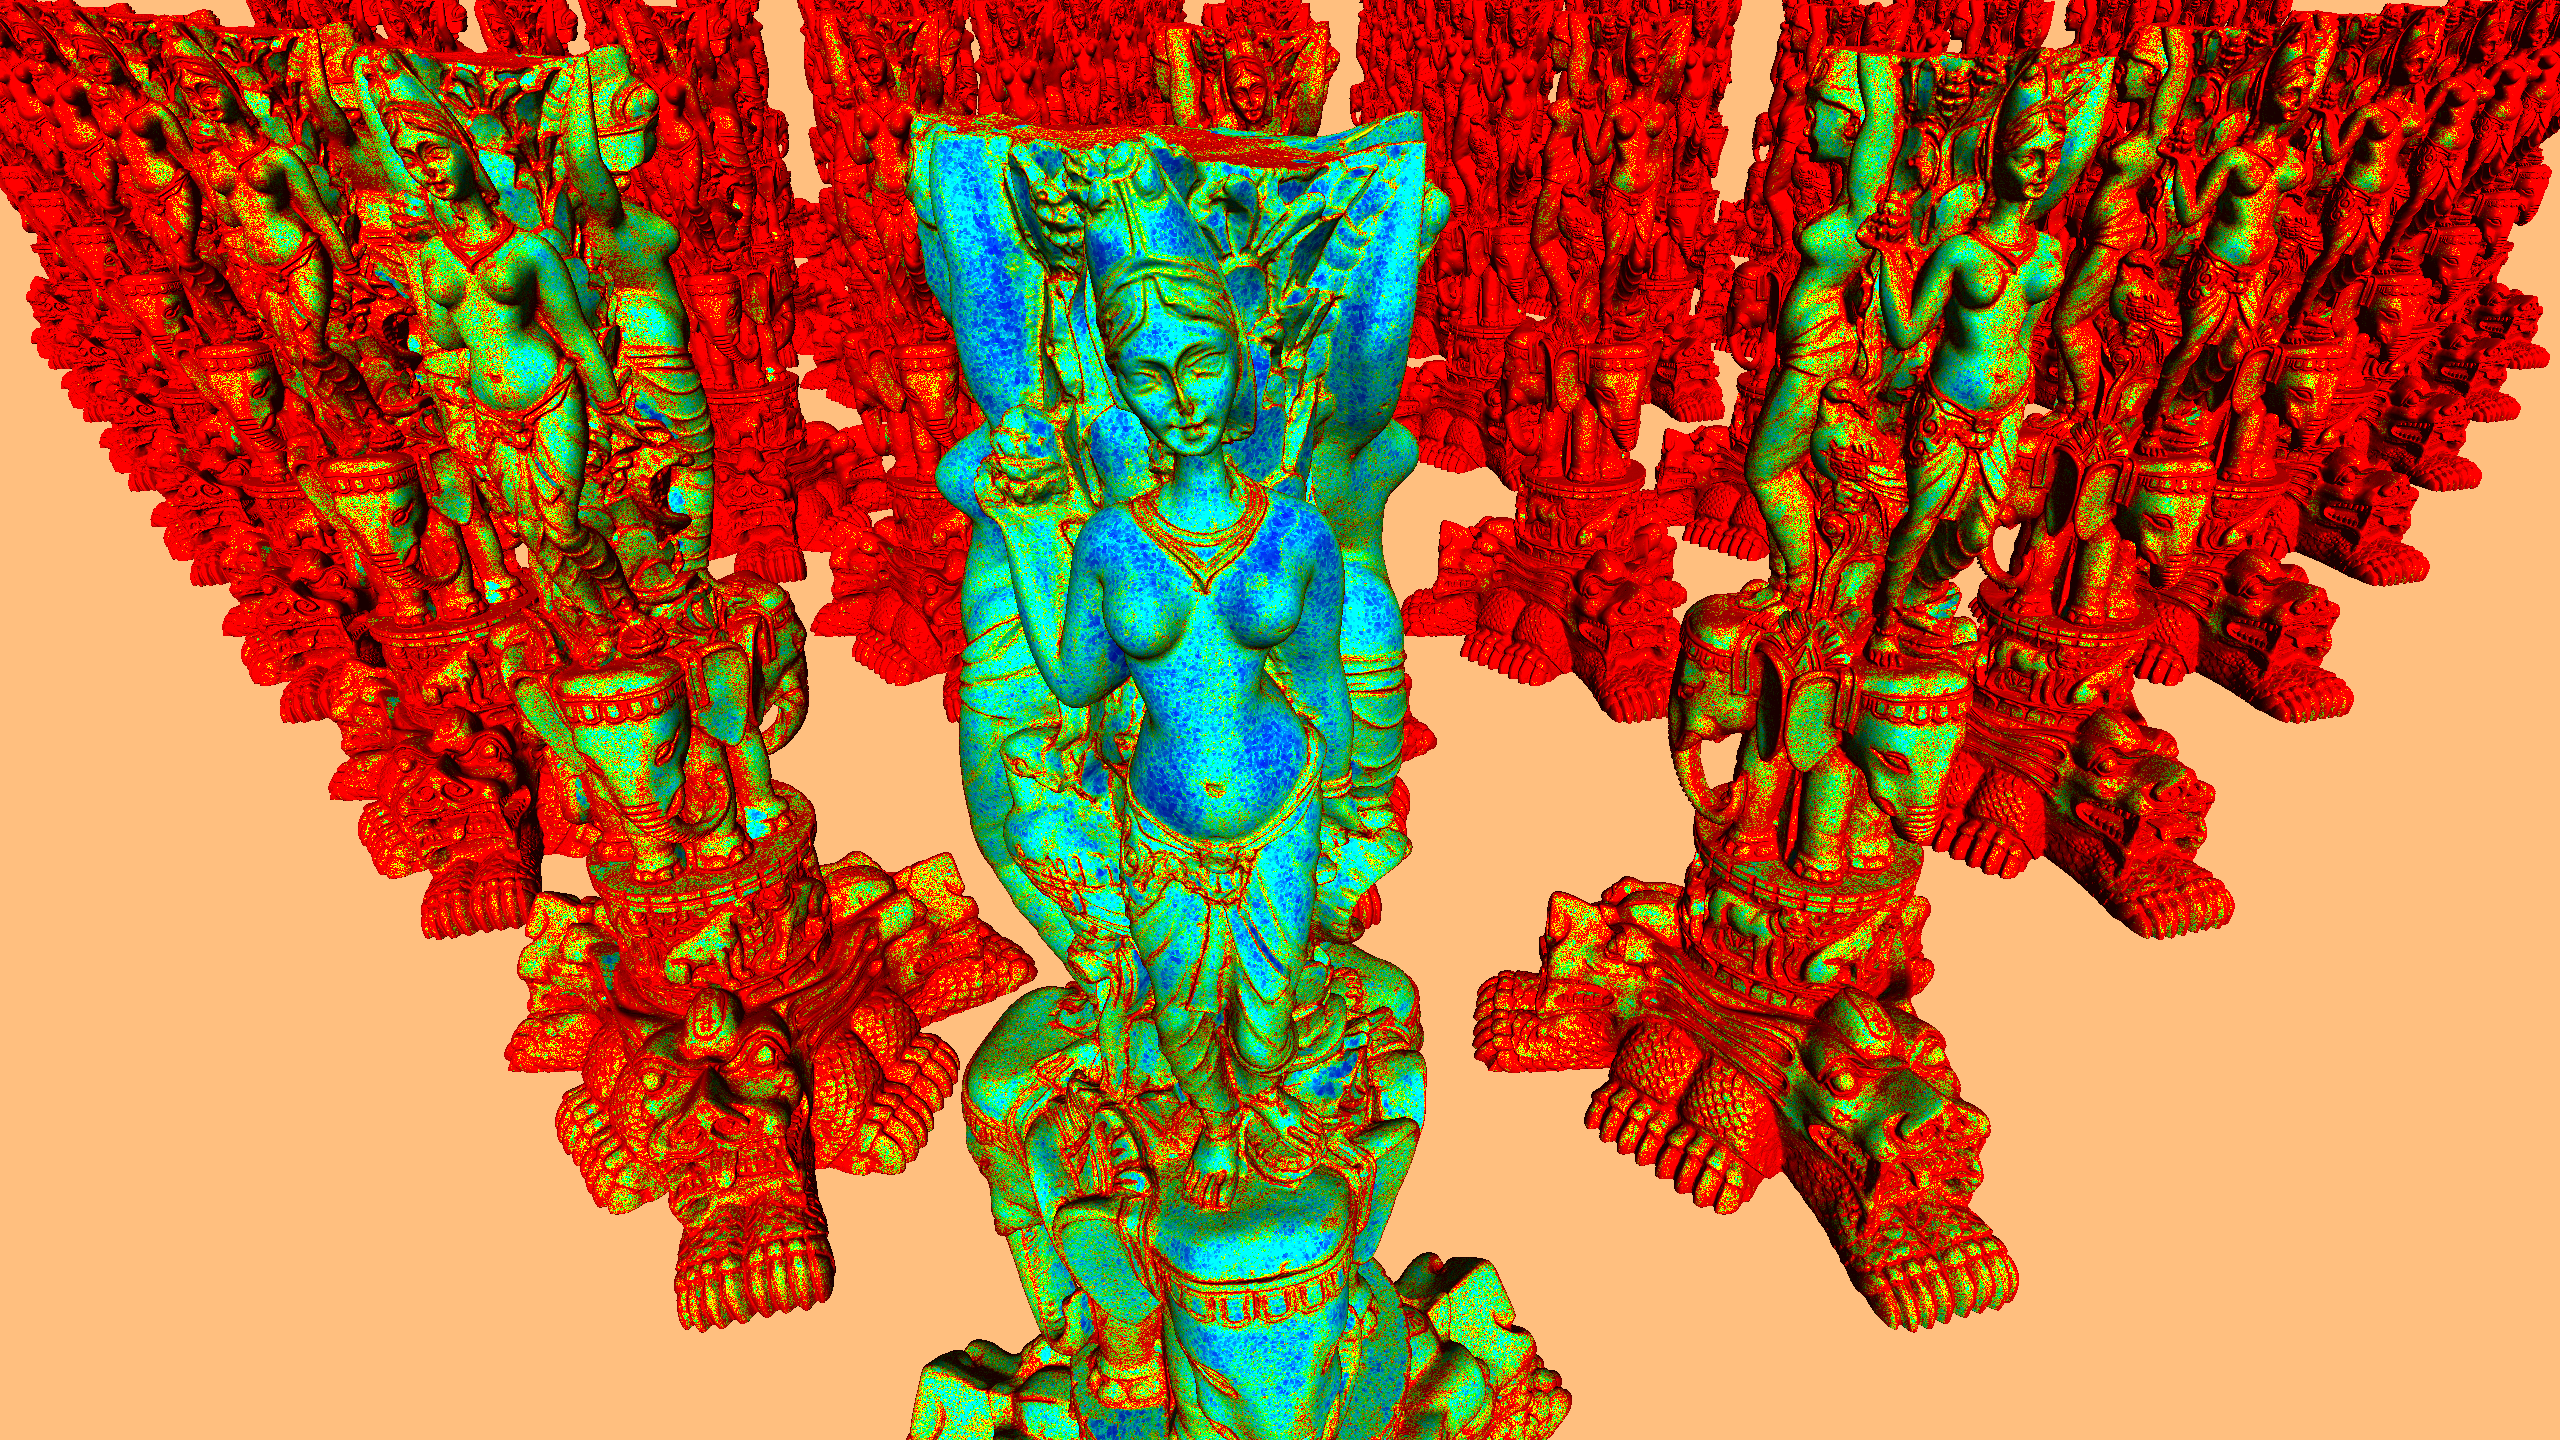
\includegraphics[width=\textwidth]{../Text/pics/heatmap-0.png}

                Наивысшая детализация
            \end{center}
        \end{minipage}
    \end{center}
\end{frame}

\begin{frame}{Доп.: Исходный код}
    Исходный код доступен в GitHub-репозитории\\
    \url{https://github.com/asurkis/MasterThesis}

    \bigskip

    \begin{center}
        \qrcode[hyperlink,height=.5\textheight]{https://github.com/asurkis/MasterThesis}
    \end{center}
\end{frame}

    \setcounter{framenumber}{\value{finalframe}}
\end{document}
